\documentclass[10pt,twocolumn,letterpaper]{article}
\usepackage{graphicx}
\usepackage{amsmath}
\usepackage{amssymb}
\usepackage{booktabs}
\usepackage{nicefrac}
\usepackage{algorithm}
\usepackage[algo2e]{algorithm2e} 
\usepackage{multirow}
\usepackage[pagebackref,breaklinks,colorlinks]{hyperref}
\usepackage{float}

% Support for easy cross-referencing
\usepackage[capitalize]{cleveref}
\crefname{section}{Sec.}{Secs.}
\Crefname{section}{Section}{Sections}
\Crefname{table}{Table}{Tables}
\crefname{table}{Tab.}{Tabs.}

\begin{document}
\nocite{*}

\title{EXAMEN}
\author{clement duny }
\maketitle

he calibrated setting? Apart from the theoretical interest,
one answer to this question concerns stability and unique-
ness of solutions. Enforcing the intrinsic calibration con-
straints often gives a crucial improvement of both the accu-
racy and robustness of the structure and motion estimates.
Currently, the standard way of achieving this is through
an initial uncalibrated estimate followed by iterative refine-
ment to bring the estimate into agreement with the calibra-
tion constraints. When the intrinsic parameters are known
a priori, the five-point algorithm is a more direct way of en-
forcing the calibration constraints exactly and obtaining a
Euclidean reconstruction. The accuracy and robustness im-
provements gained by enforcing the calibration constraints
are particularly significant for planar or near planar scenes
and scenes that appear planar in the imagery. The uncali-
brated methods fail when faced with coplanar scene points,
since there is then a continuum of possible solutions. It has
been proposed to deal with this degeneracy using model se-
lection [43, 35], switching between a homographic model
and the general uncalibrated model as appropriate. In the
calibrated setting, coplanar scene points only cause at most
a two-fold ambiguity [21, 23]. With a third view, the am-
biguity is in general resolved. In light of this, a RANSAC
scheme that uses the five-point algorithm over three or more
views is proposed. It applies to general structure but also
continues to operate correctly despite scene planarity, with-
out relying on or explicitly detecting the degeneracy. In
essence, the calibrated model can cover both the planar and
general structure cases seamlessly. This gives some hope
of dealing with the approximately planar cases, where nei-
ther the planar nor the uncalibrated general structure model
applies well.
The rest of the paper is organized as follows. Section 2
establishes some notation and describes the constraints used
in the calibrated and uncalibrated cases. Section 3 presents
the five-point algorithm. Section 4 discusses planar degen-
eracy. Section 5 outlines the RANSAC schemes for two
and three views. Section 6 gives results. The numerical ac-
curacy of the algorithm is investigated in Section 6.1. The
distribution of the number of solutions is studied in Section
6.2. Timing information is given in Section 6.3. The per-
formance of the algorithm in noisy conditions is studied in
Section 6.4, where the performance of the 5-point algorithm
is compared to that of the well known 8 and 7-point algo-
rithms and a 6-point scheme. Some reconstruction results
are given in Section 6.5. Section 7 concludes.

\section {\label{sec:Preliminaries}Preliminaries}
Image points are represented by homogeneous 3-vectors $q$
and $q'$ in the first and second view, respectively. World
points are represented by homogeneous 4-vectors Q. A per-
spective view is represented by a 3 × 4 camera matrix $P$
indicating the image projection $q\sim PQ$, where $\sim $ denotes
equality up to scale. A view with a finite projection centre
can be factored into $P = K \left[R |t\right]$, where $K$ is a 3 × 3
upper triangular calibration matrix holding the intrinsic pa-
rameters and $R$ is a rotation matrix. Let the camera matrices
for the two views be $K_1 \left[I | 0\right]$ and $P = K_2 \left[R | t\right]$. Let $[t]_\mathbf{x}$
denote the skew symmetric matrix


\begin{equation}
    \left[t\right]_\mathbf{x} =
     \left[
    \begin{array}{ccc}
    0 & -t_3 & t_2 \\
    t_3 & 0 & -t_1 \\
    -t_2 & t_1 & 0 \\
    \end{array}
    \right]
    \label{eq:eq1}
\end{equation}

{\small

}

so that $\left[t\right]_\mathbf{x}x = t\times x$ for all $x$. Then the fundamental matrix
is
\begin{equation}
   F=K_2^{-t} \left[t\right] _\mathbf{x}RK_1^{-1}
    \label{eq:eq2}
\end{equation}
The fundamental matrix encodes the well known copla-
narity, or epipolar constraint
\begin{equation}
    q^{'T}Fq=0
    \label{eq:eq3}
\end{equation}
The fundamental matrix can be considered without knowl-
edge of the calibration matrices. Moreover, it continues to
exist when the projection centres are not finite. If $K_1$ and
$K_2$ are known, the cameras are said to be calibrated. In this
case, we can always assume that the image points $q$ and $q'$
have been premultiplied by $K_1^{-1}$ and $K_2^{-1}$
, respectively, so
that the epipolar constraint simplifies to
\begin{equation}
    q^{'T}Fq=0
    \label{eq:eq4}
\end{equation}
where the matrix $E=\left[t\right]_R$ is called the essential matrix.
Any rank-2 matrix is a possible fundamental matrix, i.e. we
have the well known single cubic constraint, e.g. [14]:



\textbf{Theorem 1}\textit{ A real non-zero 3×3 matrix F is a fundamental
matrix if and only if it satisfies the equation}

\begin{equation}
    det\left(F\right)=0
    \label{eq:eq5}
\end{equation}

An essential matrix has the additional property that the two
non-zero singular values are equal. This leads to the follow-
ing cubic constraints on the essential matrix, adapted from
[38, 6, 22, 32]:

\textbf{Theorem 2}\textit { A real non-zero 3 × 3 matrix F is an essential
matrix if and only if it satisfies the equation}

\begin{equation}
    EE^TE-\frac{1}{2}trace\left(EE^T\right)E=0
    \label{eq:eq6}
\end{equation}

Both (5) and (6) will help us recover the essential matrix.
Once the essential matrix is known, $R$, $t$ and the camera
matrices can be recovered from it.


\begin{figure}[H]
    \centering
    \begin{tabular}{cc}
         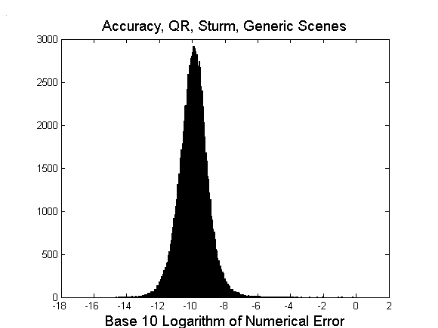
\includegraphics[width=4cm]{images/im1.png} &  
         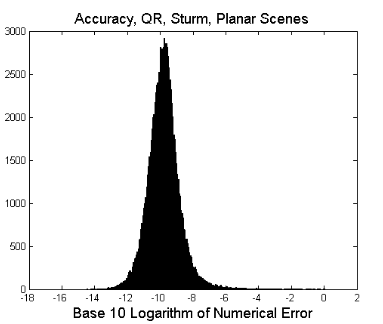
\includegraphics[width=3.5cm]{images/im2.png}  
    \end{tabular}
    \caption{ Distribution of numerical error in the essential matrix
Ê based on $10^5$ random tests. QR is used in Step 1 and Sturm-
bracketing plus root polishing in Step 5. The median error is 1.2 ·
$10^{−10}$ for generic and 1.6 · $10^{−10}$ for planar scenes. 0.1\% of the
trials for generic and 0.5\% for planar scenes had error magnitudes
above $10^{-6}$.}
    \label{fig:fig1}
\end{figure}


\bibliographystyle{IEEEtran}
\bibliography{BIBTex}
\end{document}


